\documentclass[12pt,a4paper,openright,twoside]{book}
\usepackage[utf8]{inputenc}
\usepackage{disi-thesis}
\usepackage{code-lstlistings}
\usepackage{notes}
\usepackage{shortcuts}
\usepackage{acronym}

\school{\unibo}
\programme{Corso di Laurea Triennale in Ingegneria e Scienze Informatiche}
\title{Fancy Title}
\author{Candidate Name}
\date{\today}
\subject{Supervisor's course name}
\supervisor{Prof. Supervisor Here}
\cosupervisor{Dott. CoSupervisor 1}
\morecosupervisor{Dott. CoSupervisor 2}
\session{I}
\academicyear{2023-2024}

% Definition of acronyms
\acrodef{IoT}{Internet of Thing}
\acrodef{GPIO}{General Purpose Input/Output}
\acrodef{PWM}{pulse-width modulation}
\acrodef{SBC}{Single Board Computer}
\acrodef{JS}{JavaScript}

\mainlinespacing{1.241} % line spacing in mainmatter, comment to default (1)

\begin{document}

\frontmatter\frontispiece

\begin{abstract}
    TODO
\end{abstract}

\begin{dedication} % this is optional
    Optional. Max a few lines.
\end{dedication}

%----------------------------------------------------------------------------------------
\tableofcontents
%\listoffigures     % (optional) comment if empty
%\lstlistoflistings % (optional) comment if empty

\mainmatter

\chapter*{Introduzione}
\addcontentsline{toc}{chapter}{Introduzione}  % Aggiunge l'Introduzione al sommario
\setcounter{chapter}{0}  % Resetta il contatore dei capitoli a 0


Generalmente viene scritta alla fine, non è un capitolo, racchiude un riassunto stretto del contenuto della tesi: problema -> soluzioni esistenti -> descrizione nuova soluzione -> conclusioni. Lunghezza da 1-3 .

Write your intro here.
You can use acronyms that your defined previously,
such as \ac{IoT}.
%
If you use acronyms twice,
they will be written in full only once
(indeed, you can mention the \ac{IoT} now without it being fully explained).

\paragraph{Structure of the Thesis}

\note{At the end, describe the structure of the paper}

\chapter{Precision Watering}

%Introduce il lettore alla tesi, descrive il concetto di agricoltura di precisione, perché è nata (in termini di necessità), quali obbiettivi si pone e quali sono i maggiori limiti che sta incontrando; in allegato trovi la mia tesi magistrale, sentiti pure libero di usarlo come fonte, soprattutto il primo capitolo. Lunghezza 10-15 pagine

L'argicultura è ricunosciuta come elemento fondamentale dello sviluppo della civiltà umana (fonte). L'agricultura è anche una delle industrie che più sfruttano le risorse idriche (fonte) il che contribuisce all'aumento delle temperature (fonte). Per poter affrontare la crisi climatica diventa necessario lo studio, sviluppo e utilizzo di tecnologie per limitare gli sprechi di acqua all'interno dell'agricultura, questo è l'obbiettivo del precision watering.

La sezione 1.1 (capire come fare in latex) illustra qual è l'impatto climatico dell'agricultura per quel che concerne lo sfruttamento di acqua, la sezione 1.2 mostra quali possono essere i possibili approcci all'agricultura di precisioni e infinire la sezione 1.3 ragiona su quali sono i limiti degli approcci precedentemente elencati.

\section{Necessità e obbiettivi}

riscaldamento globale, trova studi sullo spreco di acqua, trova studi in italia sulla siccità

\section{Approcci}

Sia csm che capitolo 2

\section{Limiti incontrati}

Non so se è separabile dagli approcci

\chapter{Tecnologie utilizzate}

%Descrive appunto le tecnologie utilizzate nel progetto: sia lato HW (Arduino + Raspberry + sensori), sia lato SW (stack tecnologico). Lunghezza 5-8 pagine.


\section{Hardware}

\begin{itemize}
    \item \textbf{Sensori}, TODO numero sensore e citazione alle specifiche
    \item \textbf{Arduino UNO R3} è una scheda microcontrollore basata sull'ATmega328P. Permette di caricare i programmi scritti in linguaggio C++ usando un'architettura SuperLoop, dove un unico pezzo di codice viene ripetuto fin tanto che il dispositivo è riceve alimentazione. Il superloop è interrompibile momentaneamente solo tramite degli interrupt di sistema, che vengono gestiti con routine non interrompibili, ciò implica che durante una routine, non possono avvenire altri interrupt. È quindi consigliabile che le routine di gestione siano particolarmente brevi, sia per evitare perdita di eventi, sia perchè molte librerie di sistema sfruttano internamente gli interrupt, per esempio \texttt{delay} (equivalmente a sleep di python). Offre l'utilizzo di un totale di 22 pin \ac{GPIO}: 16 dei quali digitali, di cui 6 utilizzabili come output analogici tramite \ac{PWM}, e altri 6 pin input analogico. Può inoltre gestire una comunicazione seriale tramite USB con la quale è possibile comunicare con altri dispositivi.
    \item \textbf{Raspberry Pi 4 model B} è un \ac{SBC} in grado di utilizzare sistemi operativi veri e propri basati sul kernel Linux o su RISC OS. Presenta un processore quad-core ARM a 64bit ad una velocità di clock di 1.80GHz. La configurazione utilizzata presenta \note{QUANTITARAM} Gb di RAM LPDDR4-3200. Compatibile con Bluetooth 5.0, BLE, connessioni wireless IEEE 802.11ac a 2.4 GHz e 5.0 GHz, oltre che Gigabit Ethernet. Permette anche l'utilizzo di 40 pin GPIO digitali. Compatibile con periferiche USB tramite 2 porte USB2.0 e 2 porte USB3.0. L'uscita video è permessa da tramite 2 porte Micro-HDMI, che supportano dual-screen 4k. Come storage viene utilizzata una singola scheda microSD. Include un'interfaccia MIPI DSI per display e MIPI CSI per telecamere, ed è alimentato tramite un connettore USB-C da 5V/3A. Prodotto dalla Raspberry Pi Foundation, che ha realizzato diversi modelli per varie esigenze, è compatibile con vari sistemi operativi, tra cui il più noto è Raspberry Pi OS (precedentemente chiamato Raspbian), una versione di Debian sviluppata dalla stessa fondazione.
\end{itemize}
    
\section{Software}

    \begin{itemize}
        \item \textbf{\ac{JS}} è un linguaggio di programmazione interpretato, usato principalmente per la programmazione web sia a livello client che server, per esempio con l'utilizzo di Node.js. È un linguaggio dinamico, basato sui prototipi, multi-paradigma, single-threaded , che supporta stili di programmazione orientati agli oggetti, imperativi e dichiarativi. Standardizzato come ECMAScript, \ac{JS} è alla base di un vasto ecosistema di librerie e framework che ne ampliano le capacità e l'applicabilità in diversi contesti.
        \begin{itemize}
            \item \textbf{Chart.js} è una libreria \ac{JS} semplice e flessibile per la generazione di grafici lato frontend. Si tratta di un progetto Open Source che sfrutta i canvas di HTML5. Di default permette l'utilizzo di 8 diversi tipi di grafici, è compatibile con plug-in che permettono l'aggiunta di nuove funzionalità. 
            \begin{itemize}
                \item \textbf{chartjs-chart-matrix} è un plug-in che permette la creazione di grafici a matrice, un esempio è in \cref{fig.matrix_chart_example}
                \begin{figure}
                    \centering
                    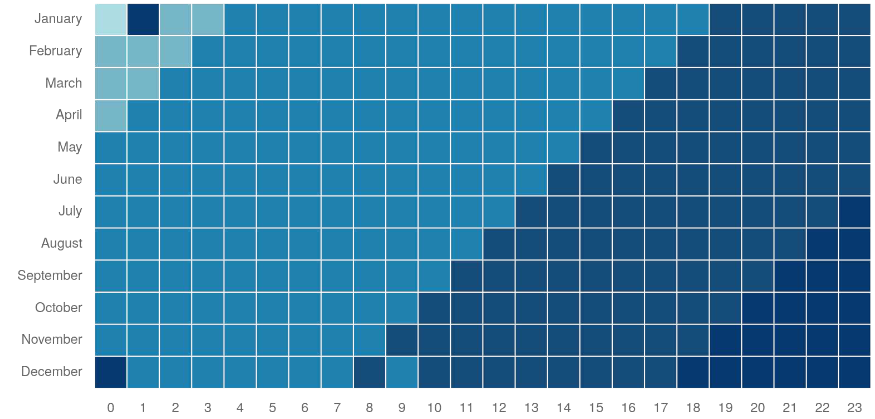
\includegraphics[width=0.9\linewidth]{./figures/matrix-chart-example.png}
                    \caption{Esempio di una mappa delle temperature medie giornaliene per mese, l'intensità del colore è proporzionale alla temperatura.}
                    \label{fig.matrix_chart_example}
                \end{figure}
                \item \textbf{chartjs-plugin-streaming} è un plug-in che permette la creazione di grafici con valori in tempo reale. Prevede lo scorrimento verso sinistra del grafico in base al tempo. È possibile configurarlo per moficare la granularità, la frequenza di aggiornamento ed un eventuale delay in modo da avere una visualizzazione "fluida" dei nuovi dati. Necessita di un adapter per una libreria per la gestione delle date e ricezione del tempo attuale, come Luxon.
                \item \textbf{chartjs-plugin-datalabels} è un plug-in per la visualizzazione dei dati su un grafico, un esempio su un grafico a linea è visibile in \cref{fig.datalabels-example}
                \begin{figure}
                    \centering
                    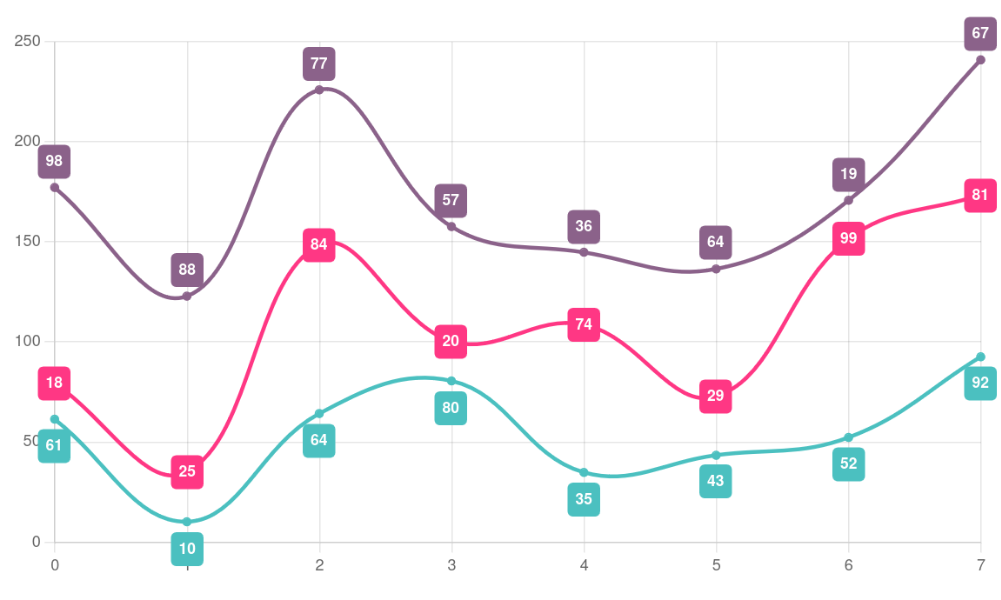
\includegraphics[width=0.9\linewidth]{./figures/datalabels-example.png}
                    \caption{Esempio utilizzo di datalabels dove in ogni linea la posizione del label è differente.}
                    \label{fig.datalabels-example}
                \end{figure}
                \item \textbf{chartjs-adapter-luxon} è un plug-in che si occupa di fornire a chartjs-plugin-streaming le informazioni sulle date da Luxon.
            \end{itemize}        
            \item \textbf{Luxon} è un wrapper di date e tempi per \ac{JS}. Utilizza un'API per gestiore le date, che consente il supporto agli intervalli, alle durate (14 days, 5 minutes, 33 seconds), la loror conversione e parsing. Offre la localizzazione delle stringhe con una gestione interna delle time-zones.
            \item \textbf{bootstrap} è un toolkit frontend potente ed estendibile. Permette la creazione di interfacce web utilizzando unicamente classi HTML, senza la necessità di scrivere il proprio foglio di stile CSS.
            \item \textbf{jQuery} è una famosa libreria per la manipolazione e navigazione di documenti HTML, la gestione degli eventi, le animazioni e richieste HTTP.
            \item \textbf{Socket.io} permette l'apertura di una comunicazione bidirezionale sempre attiva tra client e server utilizzando WebSocket. 
        \end{itemize}
        \item \textbf{Python} è un linguaggio di programmazione ad alto livello che supporta il paradigma object-oriented, la programmazione struttrata e molte caratteristiche di programmazione funzionale. È un linguaggio debolmente tipizzato, che utilizza unicamente l'indentazione per la definizione dei blocchi di codice, al contrario di molti linguaggi, non prevede quindi l'utilizzo di parentesti graffe. Supporta l'overloading di operatori e funzioni tramite delegati, oltre che sinstassi avanzate quali slicing (l'utilizzo di un certo range di elementi in una lista) e list comprehension (la creazione di nuove liste partendo da una originale). Il codice python viene interpretato (con delle compilazioni a bytecode alla prima esecuzione per migliorare le performance) che supporta anche un uso interattivo.
        \begin{itemize}
            \item \textbf{Flask} è un framework web per la creazione di backend per Python. 
            \item \textbf{Flask-SocketIO} è una libreria Python per la gestione di websocket tramite Socket.io.
            \item \textbf{NumPy} è la libreria principale per il calcolo scientifico Python. Permette la gestione di array $n$-dimensionali ed è ampiamente utilizzato per operazioni di algebra lineare, trasformate di Fourier, manipolazioni di dati e altre applicazioni numeriche. È uno strumento essenziale per chi lavora con analisi numeriche, machine learning e data science.
            \item \textbf{pySerial} è una libreria per l'accesso a porte seriali. Permette la stessa gestione delle porte seriali su ogni piattaforma. Supporta diversi byte size, bit di parità e di fine messaggio, oltre che controllo del flusso. La porta è configurata per la trasmissione binaria.
            \item \textbf{dotenv} è un modulo per la gestione delle variabili d'ambiente.
            \item \textbf{pytz} è una libreria per il calcolo del fuso orario in python.
            \item \textbf{SciPy} è una libreria di Python per il calcolo scientifico e tecnicho, espande NumPy. Offre un'ampia quantità di funzionalità per l'ottimizzazione, la statistica, l'integrazione, l'algebra lineare, l'elaborazone dei segnali, la gestione di immagini e altre operazioni matematiche avanzate. È molto utilizzata per esempio nei campi della fisica, dell'ingegneria, della biologia computazionale.
        \end{itemize}
        \item \textbf{C++} è un linguaggio di programmazione nato come espansione del linguaggio C, presenta caratteristiche di programmazione funzionale, generica e orientata agli oggetti, permettendo però una gestione a basso livello della memoria. Per quest'ultima caratteristica è tipicamente utilizzato in contesti dove le prestazioni sono particolamente importanti come lo sviluppo di sistemi operativi, software embedded, motori di gioco e applicazioni real-time. In particolar modo è utilizzanto anche per lo sviluppo di software per dispositivi con risorse limitate, come microcontrollori e sistemi embedded, dove la gestione diretta della memoria e delle risorse hardware è essenziale. 
        \begin{itemize}
            \item \textbf{Arduino API} è una libreria in C/C++ per la scrittura di codice per dispositivi Arduino. Contiene funzioni riguardanti l'hardware, per esempio, contiene funzioni per la lettura/scrittura di segnali digitali e analogici sui pin, per la gestione degli interrupt e della porta seriale. Oltre alle funzioni hardware, l'API include, ad esempio, strumenti per la gestione dei timer, funzioni matematiche, funzioni per la gestione di bit e byte e per la gestione degli stream. Contiene inoltre i tipi di variabile `enum`, `String` e funzioni per la conversione.
            \item \textbf{TimerInterrupt} è una libreria che permette l'utilizzo del timer fisico di una board Arduino come interrupt di sistema, permettendo lo svolgimento ininterrotto di ruotine periodicamente. 
            \item \textbf{ArduinoJson} è una semplice libreria per la gestione di stringhe JSON su piattaforma Arduino. Permette serializzazione e deserializzazione, ed è quindi molto utile per mandare dati strutturati sul seriale in modo che venga che lo scambio dei dati sia standardizzato.
        \end{itemize}
    \end{itemize}   



\chapter{Un prototipo di irrigazione prescrittivo}
Descrive nel dettaglio il tuo lavoro, quindi come le tecnologie presentate nella precedente sezione sono state utilizzate nel progetto. Puoi prenderla larga descrivendo il nostro sistema (quello che ti ho mostrato sul mio pc) per poi descrivere la necessità di averne una rappresentazione su piccola scala e come è stata realizzata, così come descrivere il ciclo di vita del dato (collection, processing, exploitation). Ora come ora è normale tu non abbia chiare le idee su questo capitolo, andando avanti integreremo le tue conoscenze con quelle pregresse nostre sul dominio applicativo e sul nostro sistema. Questo capitolo deve essere il core della tesi, lunghezza 20 pagine.

\chapter{Conclusioni e sviluppi futuri}

Breve capitolo che trae le conclusioni sul lavoro svolto, il risultato ottenuto rispetto a quello atteso e lo spazio dedicato a migliorie future.

%
% BIBLIOGRAPHY
%

\backmatter

\nocite{*} % Remove this as soon as you have the first citation

\bibliographystyle{alpha}
\bibliography{bibliography}

\begin{acknowledgements} % this is optional
    Optional. Max 1 page.
\end{acknowledgements}

\end{document}
